\chapter{基于本体的地理知识问答}\label{chapter:al_sup}
基于本体的地理知识问答指的是:根据构建的地理本体知识库,构建一个基于知识库的问答系统,针对用户提出的地理问题给出精准的答案。本章首先介绍本文的具体任务和系统总架构图,然后介绍地理本体知识库的具体构建方法,最后介绍基于地理本体知识库的实现流程。

\section{论文任务}
本论文任务是:根据用户提出的地理问题,系统给出该问题的简短、精准答案。如下为用户所提出的四个问题和相应回复答案举例:

(1)提问:“地球的半径大约是多少呢?”,回复:“6371km”

(2)提问:“地球半径约多少米多少千米?”,回复:“6371km”

(3)提问:“怎样保护热带雨林?”,回复:“加强环境教育,提高公民环保意识;加强雨林管理和保护,建立自然保护区;”

(4)提问:“中国采取了哪些措施保护热带雨林?”,回复:“加强环境教育,提高公民环保意识;加强雨林管理和保护,建立自然保护区;”

问题(1)、(2)问的为同一个问题,均可根据知识库中三元组“(地球,半径,6371km)”来回答。问题(3)、(4)也是问的相同问题、只是表达不同,均可根据知识库中三元组“(雨林,保护措施内容,“加强环境教育,提高公民环保意识;加强雨林管理和保护,建立自然保护区”)”来回答,系统需要区分知识库中“雨林”和问题中问的“热带雨林”其实为同一个概念。因此,本文主要有两大任务,如下:

(1)构建可以回答地理问题的地理本体知识库。

(2)在构建的地理本体知识库上构建问答系统,系统需满足用户问题按不同方式随意提问,均能正确匹配知识库中可以回答问题的答案三元组。

\section{系统结构图}
针对基于本体的地理知识问答的两大任务,本文设计了如下图\ref{fig:graduation}所示的系统总结构图。该系统结构图由三个模块组成,分别是地理本体知识库构建模块、地理问题输入、处理模块和答案选择模块。

地理本体知识库构建模块包括三个任务,第一是根据高中地理相关知识源人工构建地理本体CGeoOnt,第二将本体CGeoOnt和基于百度百科自动构建的地理本体Clinga融合成更大的本体,最后一个任务是根据融合而成的地理本体构建本体词汇表和本体同义词词汇表,简称为本体词典。

地理问题输入、处理模块包括两个任务,第一是根据地理核心知识考点,获取跟知识点相关的真实地理问题集,第二是对问题进行分析,包括问题分词、命名实体识别、词性标注和问题中包含的本体主题词识别,最终目的是生成候选答案实体供候选答案检索。

答案选择模块包括三个任务,第一是根据候选答案实体去地理本体知识库查询相应的候选答案三元组,第二是构建地理知识库问答模型对用户输入的问题和其候选答案进行向量表示,第三是根据问题和候选答案的向量表示,根据相似度打分策略和相应最终答案选择策略选取最终答案。

\begin{figure}[!htb]
	\centering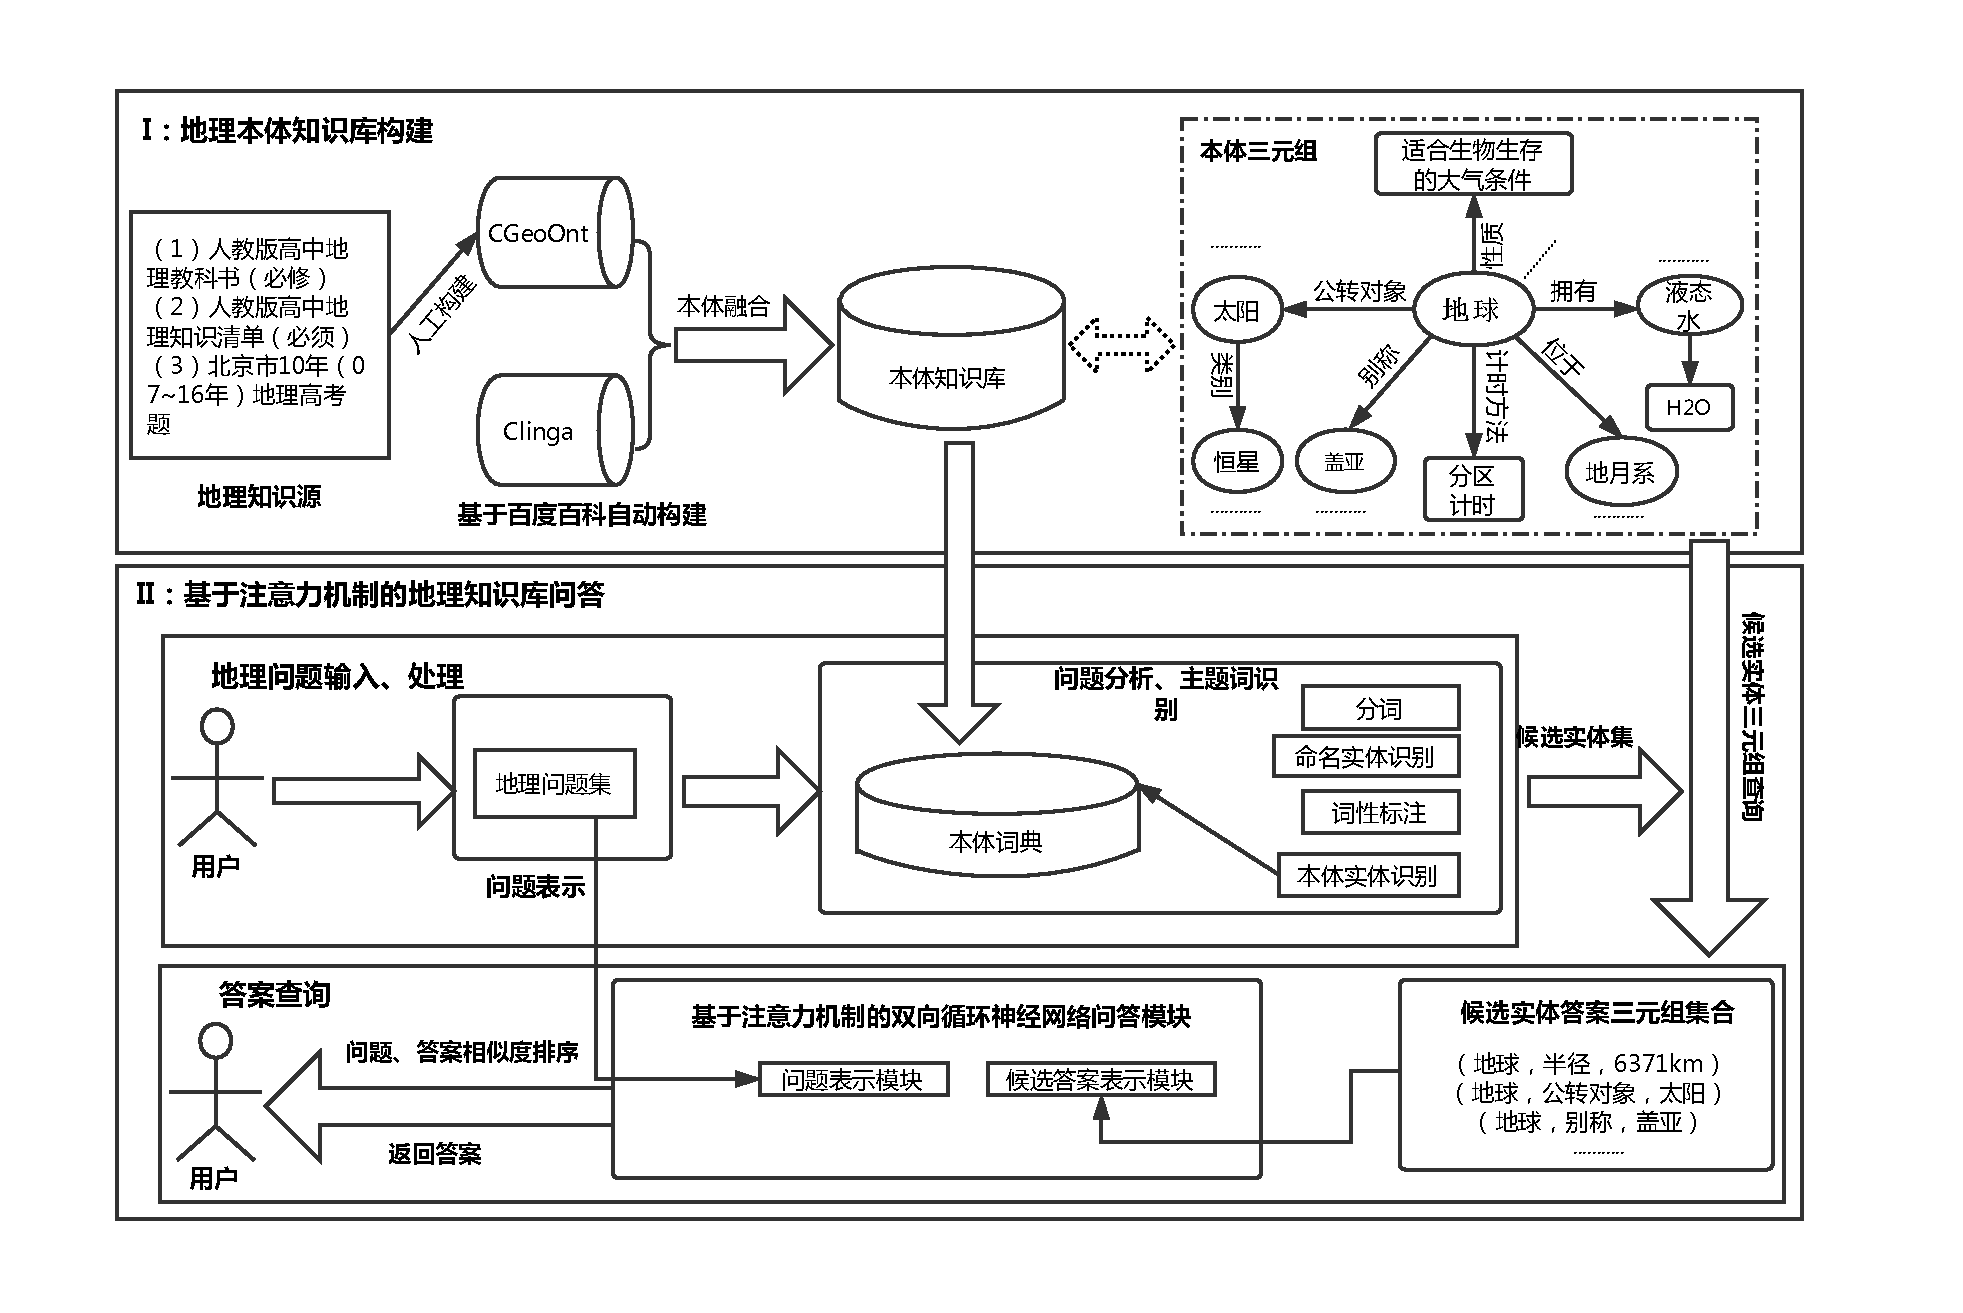
\includegraphics[height=9cm]{resource/graduation}
	\caption{基于本体的地理知识问答系统结构图}
	\label{fig:graduation}
\end{figure}

\section{地理本体知识库构建}
地理本体知识库构建内容分三个部分来介绍,先介绍地理本体CGeoOnt的构建,然后介绍本体Clinga与本体CGeoOnt融合,最后介绍本体词典生成方法。

\subsection{地理本体CGeoOnt构建}\label{section:CGeoOnt_build}
本文本体构建方法借鉴了斯坦福七步法的流程思想,但是与斯坦福的七步法有一些区别,如本文没有可以复用的本体,并且一次性列出本体的重要术语明显可操作性不强。因此,根据本文地理本体构建特点,主要分四个步骤进行构建工作,分别如下:

(1)地理知识源选取。选取本体构建所需要的资料,文档或者图形形式。

(2)地理知识体系定义。确定本体构建的三元组知识组织顺序。

(3)地理本体构建规范定义。约定本体构建的知识组织规范。

(4)地理本体基本元素定义。定义类、属性、关系,创建实例。

\subsubsection{地理知识源选取}
地理本体构建知识源来自专业的高中地理教材以及部分的高考试题。地理教材包括人教版高中地理必修一自然地理、必修二人文地理、必修三区域可持续发展、区域地理、选修三旅游地理、选修五自然灾害与防治、选修六环境保护这七本教材和一本高中地理知识清单。高中地理知识清单是专家对上述七本高中地理教材中核心考点的精确提炼以及每本书知识点的解题方法讲解。高考试题选取的是北京市近10年(2007年~2016年)的地理高考题,选取高考题作为知识源的目的是:标注人员可以根据高考题快速把握高考地理考点以及解决考点所需要的辅助知识,因此可以很有目的性的去教材中寻找需要标注的核心知识,避免标注大量对于解题无用的地理知识,大大提高了地理核心知识库构建的效率。本文地理资源均为电子资源,且格式为HTML的网页形式,里面包含文字叙述、图和表格。

\subsubsection{地理知识体系定义}
地理知识体系的定义根据《高中地理知识清单(第3次修订)》
中的组织结构进行,该高中地理知识清单包括了整个高中地理教科书中知识的组织顺序,如高中地理教材的组织先从必修地理开始,包括必修自然地理、必修人文地理、必须区域可持续发展。然后是介绍选修地理部分,包括选修旅游地理、选修自然灾害与防治和选修环境保护。对于每一本教材中的知识体系根据书中每个章节的相关主题、相关知识点和相关方法三个方面来组织,这样的好处是使知识库的知识都能够找到其知识的出处,便于后续分析知识之间的关系和知识溯源,保留知识的完整性。如在标注概念类“天体”的知识三元组时,需要标注出“天体”在书中所属的“相关主题”是“宇宙中的地球”,以及“天体”涉及的“相关知识点”是“地球的宇宙环境”和跟“天体”相关联的“相关方法”是“天体类型的判断方法”。

\subsubsection{地理本体构建规范}
地理本体构建规范主要为保证最终本体的构建形式一致,因为本体构建需要多个专业人员参与,不同人的标注主观性很大,必须经过统一的规范约束。首先,本文地理知识需要较强的表达能力且还需具备很强的推理能力,因此本文约定本体描述语言使用OWL,构建符合RDFS和OWL DL级别规范。其次,由于本文地理本体构建有很多自己的特殊定义,有些定义需要突破OWL DL的规范,因此本文构建工作不使用当前存在的本体构建工具,如protege等,本文直接以RDF三元组的语法形式Turtle\footnote{https://www.w3.org/TR/turtle/}来表示每条本体知识(三元组)。最后,本文规定个体、类、属性等的命名说明规范,统一本体的最终表现形式。

为简化三元组的表示,本文定义了本文地理本体术语的命名空间,包括自定义的三个地理本体元素——个体、属性及类的命名空间gsr、gss、gso,以及包括七个常见的本体元素命名空间:rdf、rdfs、owl、skos、xs、op和fn。以上命名空间如下所示:

% 用s表示正常的字符宽度,l代表稍微窄的字符宽度

@prefix gsr:\hphantom{sss}<http://ws.nju.edu.cn/geoscholar/resource>.

@prefix gss:\hphantom{sss}<http://ws.nju.edu.cn/geoscholar/staticOntology>.

@prefix gso:\hphantom{ssl}<http://ws.nju.edu.cn/geoscholar/ontology>.

@prefix rdf:\hphantom{sss}<http://www.w3.org/1999/02/22-rdf-syntax-ns>.

@prefix rdfs:\hphantom{ss}<http://www.w3.org/2000/01/rdf-schema>.

@prefix owl:\hphantom{ss}<http://www.w3.org/2002/07/owl>.

@prefix skos:\hphantom{ll}<http://www.w3.org/2004/02/skos/core>.

@prefix xs:\hphantom{sssl}<http://www.w3.org/2001/XMLSchema>.

@prefix op:\hphantom{ssll}<http://www.w3.org/2002/08/xquery-operators>.

@prefix fn:\hphantom{sssl}<http://www.w3.org/2005/xpath-functions>.\linebreak[3]
\\
以下为其他约定,核心思想为本体不同元素有区分度,同时见其英文名可知其中文义:
\begin{itemize}
	\item {个体:以“R\_”开头,如gsr:R\_太阳。
	}
	\item {类:以“C\_”开头,如gso:C\_天体。
	}
	\item{属性(静态属性):以“P\_”开头,两个属性owl:ObjectProperty、owl:DatatypeProperty分别以“P\_o\_”和“P\_d\_”开头。如gso:P\_o\_公转对象,gso:P\_d\_高度。
	}
	\item{个体必须声明类别owl:Class、属性必须确定是对象属性owl:ObjectProperty还是数据类型属性owl:DatatypeProperty。
	}
	\item{每个术语有且仅有一个skos:prefLabel,但是可以有多个skos:altLabel用于别名。
	}
	\item {每个术语有必要时使用skos:definition给出其定义,使用rdfs:comment对其重要方面进行评论。
	}
	\item {术语间多使用gso:relatedTo来表达它们有一定的关联性。
	}
	\item {为避免处理的复杂性,三元组中不使用空白节点( blank node )。
	}
\end{itemize}

\subsubsection{地理本体基本元素定义}

\subsection{实体链接特征}\label{section:superised_feature}
在给定指称项$m$和指称项对应的候选实体集$E_m=\{e_1,e_2,...,e_n\}$后,计算模型的输入特征:

\begin{enumerate}
	\renewcommand{\labelenumi}{(\theenumi)}
	\item {候选实体$e_i$在知识库中的先验概率,$PriorInKB(m,e_i)$,该特征的定义如公式\ref{eq:popinkb}所示。
		
		\begin{equation}\label{eq:popinkb}
		PriorInKB(m,e_i)=\frac{count(e_i)}{\sum_{e_i\in E_m} {count(e_k)}}
		\end{equation}
		
		其中,$count(e)$表示实体$e$在知识库中作为锚文本出现的次数。
	}
	\item {指称项上下文与候选实体对应词条摘要的文 本相似度,$ContextSimilarity(m,e_i)$,该特征的定义如公式\ref{eq:contex_similarity}所示。
		
		\begin{equation}\label{eq:contex_similarity}
		ContextSimilarity(m,e_i)=\frac{coocurence(m,e_i)}{length(m)}
		\end{equation}
		
		其中,$coocurence(m,e_i)$表示指称项$m$上下文和候选实体$e_i$对应知识库中摘要文本相同的单词数,$length(m)$表示指称项$m$的上下文长度。
	}
	\item {带标注样本集中,候选实体$e_i$的流行度,$PopInCorpus(e_i)$,该特征会随着人工标注的进行而产生变化。该特征的定义如公式\ref{eq:pop_in_corpus}所示。
		
		\begin{equation}\label{eq:pop_in_corpus}
		PopInCorpus(e_i)=\frac{\sum_{anno \in Corpus} {I(anno.e,e_i)}}{sizeof(Corpus)}
		\end{equation}
		
		其中,$anno$表示已标注语料中的一条标注记录,$anno.e$表示标注记录的目标实体。$I(e_i,e_j)$是示值函数,实体$e_i$和实体$e_j$相同则为1,否则为0。$sizeof(Corpus)$表示已标注指称项个数。
	}
	\item{带标注样本集中,候选实体$e_i$作为指称项$m$的目标实体的先验概率,$Prior(m,e_i)$,同上,该特征也会随着标注的进行而产生变化。该特征的定义如公式\ref{eq:prior}所示。
		
		\begin{equation}\label{eq:prior}
		Prior(m,e_i)=\frac{\sum_{anno \in Corpus} {I(anno.e,e_i)\times I(anno.m,m)}}{\sum_{anno \in Corpus} {I(anno.m,m)}}
		\end{equation}
		
		其中,$anno.e$的定义同上。$anno.m$表示标注记录$anno$的指称项。
	}
	\item 指称项名字和候选实体标题的编辑距离,$EDSimarity(m,e_i)$。该特征的定义如公式\ref{eq:ed_simarity}所示。
	
	\begin{equation}\label{eq:ed_simarity}
	EDSimarity(m,e_i)=
	\left\{
	\begin{array}{rcl}
	1       &      & {|length(m)-length(e_i)|=ED(m,e_i)}\\
	0    &      & {\text{其它}}
	\end{array} \right.
	\end{equation}
	
	编辑距离$ED(\cdot,\cdot)$是指两个字符串进行转换时,需要的字符级最少操作次数。编辑距离相似度能够检测指称项和候选实体之间的别名、缩略名等关系。
\end{enumerate}

\subsection{目标实体预测}
在使用监督学习模型$C$处理实体链接任务时,首先需要训练模型$C$。训练样本由带标注的指称项集合构成,例如,带标注的指称$m$包含$n$个候选实体,指称$m$的目标实体是$e^*$,任意一个候选实体$e_i$和指称项$m$组成一 个样本对$\left\langle m,e_i\right\rangle $,若$e_i$是目标实体$e^*$,样本对标记为正例,否则标记为反例。用所有带标注的样本对训练得到模型$C$。

训练得到模型$C$后,对于未标注指称$m$及其候选实体集$E_m$,根据上一节的计算方法获得所有候选实体和指称项组成的样本对的特征向量,模型$C$根据输入的特征向量,计算每个候选实体是目标实体的概率$P_C(e_i|m)$。该预测概率的计算方式和模型的选择相关,例如选择支持向量机模型,可以用样本点距离分类超平面的距离估计正确分类的概率\cite{李航2012统计学习方法};选择人工神经网络模型,可以对输出层每个节点的权值做$softmax$处理,以此获得每个分类标签的分类预测概率\cite{ravuri2016comparative},在此不再一一例举其它模型的预测概率估计方法。取概率最高的候选实体作为指称项$m$的预测实体,如公式\ref{eq:hat_cancidate}所示。

\begin{equation}\label{eq:hat_cancidate}
\hat{e}=\argmax_{e_i\in E_m} P_C(e_i|m)
\end{equation}

然后将该预测实体被正确划分的概率作为指称$m$被正确链接的概率,如公式\ref{eq:predict_prob}所示。

\begin{equation}\label{eq:predict_prob}
P_C(\hat{e}|m)=\max_{e_i\in E_m}P_C(e_i|m)
\end{equation}

\section{实体链接的主动学习算法}
为了减少人工标注的工作量,本文采用基于池的主动学习方法(Pool-based Active Learning)选择实体链接的待标注指称项。主动学习流程图如图\ref{fig:al_overview}所示。

\begin{figure}[!htb]
	\centering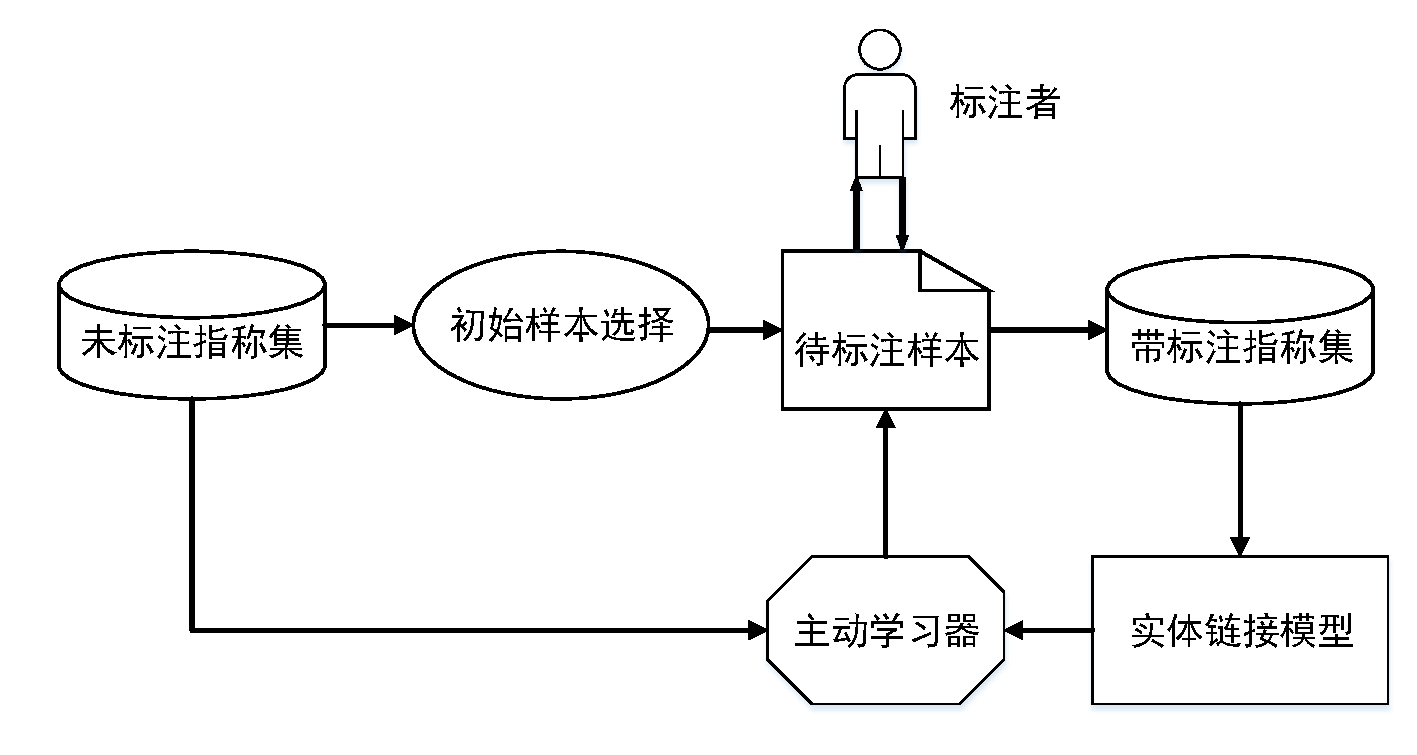
\includegraphics[height=7cm]{resource/al_overview}
	\caption{主动学习流程概览}
	\label{fig:al_overview}
\end{figure}

在每轮迭代训练中,主动学习器能够选出信息量最大的未标注样本集交由人工标注。已有的主动学习\cite{settles2012active}流程如算法\ref{algorithm_AL}所示。在给定未标注训练样本集后, 主动学习进程分为两个阶段,第一阶段的工作是选择初始训练样本集并以此训练初始分类器,第二阶段的工作是选择最佳标注样本并以此迭代训练模型。

\floatname{algorithm}{算法}
\renewcommand{\algorithmicrequire}{\textbf{输入:}} % Use Input in the format of Algorithm
\renewcommand{\algorithmicensure}{\textbf{输出:}} % Use Output in the format of Algorithm
\begin{algorithm}[!htb]
	\caption{基于主动学习的实体链接任务训练进程}
	\label{algorithm_AL}
	\begin{algorithmic}[1] %这个1 表示每一行都显示数字
		\REQUIRE ~ %算法的输入参数:Input
		未标注的指称样本集$ \mathcal{U}=\{m^{(u)} \}_{u=1}^U $
		\ENSURE ~ %算法的输出:Output
		实体链接分类器$C$
		\STATE 从未标注训练集$\mathcal{U}$中选择并标注初始训练样本集$\mathcal{L}_0$\label{al_sup_line1}
		\STATE 利用初始训练样本集$\mathcal{L}_{0}$训练得到弱分类器$C=train(\mathcal{L}_{0})$\label{al_sup_line2}
		\REPEAT \label{al_sup_line3}
		\STATE 从$\mathcal{U}$中找出$k$个信息量最大的样本组成样本集$ \mathcal{U}_{selected} = \{m^{(u)} \}_{u=1}^{k} $\label{al_sup_line4}
		\STATE 对$ \mathcal{U}_{selected}$中的指称进行人工标注得到$ \mathcal{L}_{selected} = \{\left\langle m,e\right\rangle^{(l)} \}_{l=1}^{k} $
		\STATE $ \mathcal{U} = \mathcal{U} \setminus \mathcal{U}_{selected} $
		\STATE $ \mathcal{L}_{t+1} = \mathcal{L}_{t} \cup \mathcal{L}_{selected} $
		\STATE $C=train(\mathcal{L}_{t+1})$
		\UNTIL {达到预期精度或样本集已全部标注} \label{al_sup_line9}
		\RETURN $C$
	\end{algorithmic}
\end{algorithm}

算法第\ref{al_sup_line1}-\ref{al_sup_line2} 行对应主动学习进程的第一个阶段,已有的做法是在未标注样本集$\mathcal{U}$中随机选择待标注样本$\mathcal{U}_{selected}$,然后对这些未标注样本进行人工标注,通过这种方式得到初始带标注样本集$\mathcal{L}_0$,然后用$\mathcal{L}_0$训练得到初始实体链接模型$C$。由于当初始带标注样本集合较小时,通过随机选择的方式获得的子样本集可能无法很好地代表整个样本集。因此,本文对初始训练样本选择方法做了改进,提出基于指称项流行度的初始样本选择方法。

算法第\ref{al_sup_line3}-\ref{al_sup_line9} 行对应主动学习的第二个阶段,其中对于算法第\ref{al_sup_line4}行 信息量度量方法的选择,已有的做法是将样本分类结果的不确定度大小作为信息量的衡量标准,第$t$轮迭代中选出的样本会被加入到带标注样本集$\mathcal{L}_t$中,然后用$\mathcal{L}_t$重新训练模型。在实体链接任务中,仅将不确定度作为选择待标注样本的依据,可能会导致选择过多的离群样本点,不利于模型的训练。因此,本文对迭代训练样本选择方法做了改进,提出综合分类不确定度和指称项流行度的迭代训练样本选择方法。

\section{改进的初始训练样本选择方法}\label{section:al_init_gen}
本节首先对改进的初始训练样本选择方法进行了详细说明,然后给出了该方法对应的算法描述。

\subsection{初始训练样本选择方法}
在主动学习的初始阶段,需要产生一个初始样本集用于训练初始模型。已有的主动学习方法采用随机选择的方式产生初始训练样本集,由于训练样本集相对较小,随机选择的方式很难保证初始样本集的代表性。但是,训练一个性能较好的初始模型对提高主动学习收敛速度非常重要。因此,本文对已有的基于随机选择的初始样本集生成方法做了改进。

为了提高实体链接初始模型的性能,本文提出基于流行度的初始样本选择方法(Sampling by Popularity, SBP)。指称项的流行度按照相同名字的指称项在语料库中出现的频率计算。例如,语料库中包含$n$个指称项,名字为“Jordan”的指称项出现了$m$次,则名字为“Jordan”的所有指称项的流行度为$m/n$。该样本选择方法首先对指称项按照指称项名字分类,计算指称项流行度,然后对指称项流行度高的样本做标注,加入初始训练样本集。该方法的目的是在初始样本选择阶段,尽量选择出现频率较高的指称项,以此保证初始样本集的代表性,从而提高在初始样本集较小的情况下,尽可能提高初始模型的性能。

\subsection{初始训练样本选择算法}
算法\ref{algorithm_init}是对基于流行度的初始样本选择方法的算法描述。初始训练样本的选择分为两个步骤,第一步是不同指称项流行度的统计;第二步是根据指称项流行度选择初始训练样本。

算法第\ref{al_init_line1}-\ref{al_init_line2}行对未标注样本集按指称项名字进行分类,例如所有指称名字为“Jordan”的训练样本都会被划分到集合$\Psi_{Jordan}$中。然后根据集合中的样本数量计算各个指称项在训练集中的流行度,指称项名字相同的样本具有相同的流行度。

算法第\ref{al_init_line3}-\ref{al_init_line7}行对指称项流行度做排序,并在流行度最高的$k$个样本集中分别随机选择一个或多个\footnote{当指称名字数量小于$k$时,需要在一个类簇中选择多个样本,保证最终获得$k$个样本。}样本,经过人工标注后加入初始训练样本集。这样做的目的在于避免初始训练样本集中的样本指称项名字重复度过高,同时保证尽量选择流行度高的指称项样本,从而提高初始训练样本集的代表性。

\floatname{algorithm}{算法}
\renewcommand{\algorithmicrequire}{\textbf{输入:}} % Use Input in the format of Algorithm
\renewcommand{\algorithmicensure}{\textbf{输出:}} % Use Output in the format of Algorithm
\begin{algorithm}[!htb]
	\caption{基于流行度的初始样本集选择算法}
	\label{algorithm_init}
	\begin{algorithmic}[1] %这个1 表示每一行都显示数字
		\REQUIRE ~ %算法的输入参数:Input
		未标注的实体链接样本集$ \mathcal{U}=\{m^{(u)} \}_{u=1}^U $,初始训练集样本个数$k$
		\ENSURE ~ %算法的输出:Output
		初始样本集$\mathcal{L}$
		\STATE 对未标注训练样本按照指称名字$name$分组,指称名字为$name$的样本被分到集合$\Psi_{name}$中\label{al_init_line1}
		\STATE 计算名字为$name$的指称的流行度$\Phi_{name}=\frac{|(\Psi_{name})|}{U}$\label{al_init_line2}
		\STATE 对不同指称的流行度排序,取流行度最高的$k$个指称的名字\label{al_init_line3}
		
		$\mathcal{S}=\{name_1,name_2,...,name_k\}$\label{al_init_line4}
		\FOR {each $name$ in $\mathcal{S}$}
		\STATE 从集合$\Psi_{name}$中随机取一个或多个样本并对其人工标注得到带标注的样本对$L=\left\langle m,e\right\rangle$\label{al_init_line5}
		\STATE $\mathcal{L}=\mathcal{L} \cup \{L\}$
		\ENDFOR\label{al_init_line7}
		\RETURN $\mathcal{L}$
	\end{algorithmic}
\end{algorithm}

\section{改进的迭代训练样本选择方法}\label{section:al_iter_train}
本节首先对改进的迭代训练样本选择方法进行了详细说明,然后给出了该方法对应的算法描述。

\subsection{迭代训练样本选择方法}
在初始训练集上训练得到初始模型后,需要迭代选择信息量最大的未标注样本做标注,然后对模型做重新训练。在已有的主动学习迭代训练样本选择过程中,通常将不确定度最大的样本作为信息量最大的样本,这些样本会交由人工标注并加入下一轮迭代训练,通过这种方式迭代逼近真实模型。本文采用间隔(Margin)度量未标注样本的不确定度。

如公式\ref{eq:margin_confidence}所示 ,$e^{*1}$和$e^{*2}$分别表示在当前模型$C$中,给定指称项$m$,对应置信度最高的和次高的候选实体,以这两个候选实体的置信度差的绝对值作为指称$m$链接到正确实体的置信度。

\begin{align}\label{eq:margin_confidence}
\begin{aligned}
Confidence(m)&=P_C(e^{*1})-P_C(e^{*2})\\
\text{其中,\quad\quad\quad\quad\quad\quad\quad\quad\quad\quad\quad\quad}&\text{\quad\quad\quad\quad\quad\quad\quad\quad\quad\quad\quad\quad\quad\quad\quad\quad}\\
e^{*1}&=\argmax_{E_i\in E_m}P_C(e_i|m)\\
e^{*2}&=\argmax_{E_i\in E_m \setminus \{e^{*1}\}} P_C(e_i|m)
\end{aligned}
\end{align}

易知,$Confidence(m)$越小,表示模型$C$越难正确地从候选实体$e^{*1}$和候选实体$e^{*2}$中区分出目标实体,因此,指称项$m$被正确链接的置信度越小,指称项被正确链接的不确定度越大。指称项链接的不确定度如公式(\ref{eq:margin_uncertainty})所示。

\begin{equation}\label{eq:margin_uncertainty}
Uncertainty(m)=1-Confidence(m)\\
\end{equation}

在本文的实体链接任务中,如果采用仅基于不确定度的样本选择方法来选择待标注样本,则会存在两个缺陷。第一,存在一些不确定度较大,但是在所有样本中处于边缘位置的样本,这些离群样本点不具有代表性,相反还可能会对模型的训练产生负作用,在样本选择过程中,应该尽量避免这类样本点;第二,本文实体链接模型的输入特征向量包含已标注语料中候选实体流行度($PopInCopus(e_i)$)和已标注语料中候选实体先验概率($Prior(e_i|m)$)这两个特征维度,这两个特征都是在已标注样本集上通过统计得到的,因此,带标注的样本分布越离散,带标注样本集中包含的指称项和实体越多,那么上述两个特征维度的统计量越具有代表性。从这个角度看基于不确定度的样本选择算法对这两个特征的计算可能会产生负面影响。因此主动学习的样本选择策略需要在不确定度和多样性之间取一个权衡。为了解决这个问题,本文提出综合不确定度和流行度的样本选择方法(Sampling by Uncertainty and Popularity, SUP)。

\subsection{综合不确定度和流行度的样本选择算法}
接下来给出综合不确定度和流行度的样本选择方法的算法描述。SUP算法是对不确定度和多样性的折衷,如算法\ref{algorithm_iter}所示。

\begin{algorithm}[htb]
	\caption{综合不确定度和流行度样本集选择算法}
	\label{algorithm_iter}
	\begin{algorithmic}[1] %这个1 表示每一行都显示数字
		\REQUIRE ~ %算法的输入参数:Input
		未标注的实体链接样本集$ \mathcal{U}=\{m^{(u)} \}_{u=1}^U $\\
		\quad \quad 选择标注的样本个数$k$
		\ENSURE ~ %算法的输出:Output
		本轮选择标注的训练样本集$ \mathcal{L} $\\
		\STATE $ \mathcal{L} = \{\} $
		\STATE 用K-means聚类法将未标注训练样本集按照指称的流行度划分为$k$类,$Clusters=\{\Psi_1,\Psi_2,...,\Psi_k\}$\label{al_iter_line2}
		\FOR {each $\Psi_i$ in $Clusters$}
		\STATE $m^{*}=\argmax_{m \in \Psi_i} Uncertainty(m)$\label{al_iter_line4}
		\STATE 对$m^{*}$人工标注,得到$\left\langle m^{*},e\right\rangle$
		\STATE $\mathcal{L}=\mathcal{L} \cup \{\left\langle m,e\right\rangle\}$
		\ENDFOR
		\RETURN $ \mathcal{L} $
	\end{algorithmic}
\end{algorithm}

算法第\ref{al_iter_line2}行将所有未标注样本集中的指称项按照指称项流行度进行聚类,完成聚类后,同一个类簇的样本流行度相近。

算法第\ref{al_iter_line4}行从各个流行度的类簇中分别选出不确定度最大的样本交由人工标注,这里不确定度的计算方式依然是模型预测的最优候选实体和次优候选实体置信度的间隔。该样本选择算法能够保证各个指称项流行度区间的样本都有均等机会被选中标注,同时又能保证在每个类簇中被选中标注的样本都是这个类簇中不确定度最大的样本,在兼顾所选样本集多样性的同时保证了不确定度。

\section{实验结果与分析}
本节介绍主动学习方法在实体链接模型训练中的实验,说明实验环境、实验所用数据集、评价指标以及实验配置,最后给出了实验结果数据,并对实验结果进行了分析。

\subsection{实验环境}\label{section:dev_env}
硬件环境:

\begin{itemize}
	\item CPU: Intel(R) Core(TM) i7-3770 CPU @ 3.40GHz
	\item Memory: 4$\times$8GB DDR3 1333 ECC
\end{itemize}

软件环境:

\begin{itemize}
	\item CentOS Linux release 7.3.1611 (Core)
	\item IntelliJ IDEA 2016.3
	\item Java 1.8
	\item MySQL 5.6
\end{itemize}

开源工具:

\begin{itemize}
	\item LibSVM\footnote{用于实现支持向量机。}
	\item Weka 3.6\footnote{用于配合LibSVM实现支持向量机训练。}
	\item Stanford NLP\footnote{用于实现英文分词及词干抽取。}
\end{itemize}

\subsection{实验数据集}\label{section:dataset}
本文使用的数据集是在\textit{CoNLL'03}的基础上做了实体链接标注的\textit{Aida}数据集。数据集包含 1393 篇文章和28815个可用指称项。本文取20000个指称项作为训练集,其余的指称项作为测试集。

\subsection{评价指标}
本章研究主动学习在实体链接模型训练中的作用,并验证本文提出的基于流行度的初始样本选择方法以及综合不确定度和流行度的迭代训练样本选择方法对减少人工标注样本工作量的效果。实际上数据集中的指称项都已经标注好对应的目标实体,但是在模型训练过程中,本文不直接使用 Aida 数据集的标注结果,只有通过主动学习方法选择的样本的标注结果才会被使用,以此来模拟人工标注的过程。本章实验分为以下两个方面:

(1) 以随机选择方法为基线方法,评价基于流行度的初始样本选择方法在标注相同数量样本的前 下,对初始模型性能提升的效果。

(2) 以随机选择法为基线方法,评价基于不确定度的样本选择方法以及综合不确定度和流行度的样本选择方法对模型训练收敛速度的提升效果。

本文对各种样本选择方法好坏的评价指标为主动学习过程中,由主动学习器选择的训练样本所训练得到的模型在测试集里的性能表现,性能表现体现在测试集上实体链接的正确率,计算方法如公式\ref{eq:sup_al_p}所示。

\begin{equation}\label{eq:sup_al_p}
\text{准确率}(P)=\frac{\text{测试集中被正确链接的指称项个数}}{\text{测试集中所有指称项个数}}\times 100\%
\end{equation}

\subsection{模型选择}
本章使用监督学习模型处理实体链接任务,并将该任务作为分类问题来处理。在常用的机器学习分类器中,SVM模型\cite{li2016linking}是目前分类效果较好的模型,其可以通过核函数(本文使用径向基函数(Radial Base Function, RBF))将非线性可分的输入空间的特征映射到高维线性可分的空间的特征,以此学习非线性可分模型。此外,样本点距离分类超平面的远近可以作为分类置信度的依据,而主动学习过程中,分类置信度恰好是样本选择策略的考虑因素之一。

综上,本文在实验阶段使用 SVM 模型作为监督学习模型的代表,处理实体链接任务并研究主动学习方法在该任务上发挥的作用。

\subsection{初始训练样本选择方法实验}
为了验证基于指称项流行度的初始训练样本选择方法对提高初始模型性能的效果,在实验环节,分别通过基于随机选择方法(Random)和基于流行度选择方法(SBP)得到初始样本集,对比在不同初始训练样本集大小的情况下,由初始样本集训练得到的初始模型的性能。

实验中,初始样本集大小的设置从 2000 开始,依次以 2000 递增,最大的初始样本集包含 18000 个训练样本。从图\ref{fig:al_sup_init_result}可以看出,在初始样本集较小的时候,基于指称项流行度的样本选择方法比随机样本选择方法在初始模型的性能上有显著的提升,在初始样本集大小为 2000 的时候,性能提升了 10.1\%,在初始样本集大小为 4000 的时候,性能提升了 5.3\%。当初始样本集大小继续增加时,性能提升值逐渐减小,甚至在一些情况下提升值为负。总体来看,当初始样本集较大时,两种初始训练样本选择方法性能差别不大。

\begin{figure}[!htb]
	\centering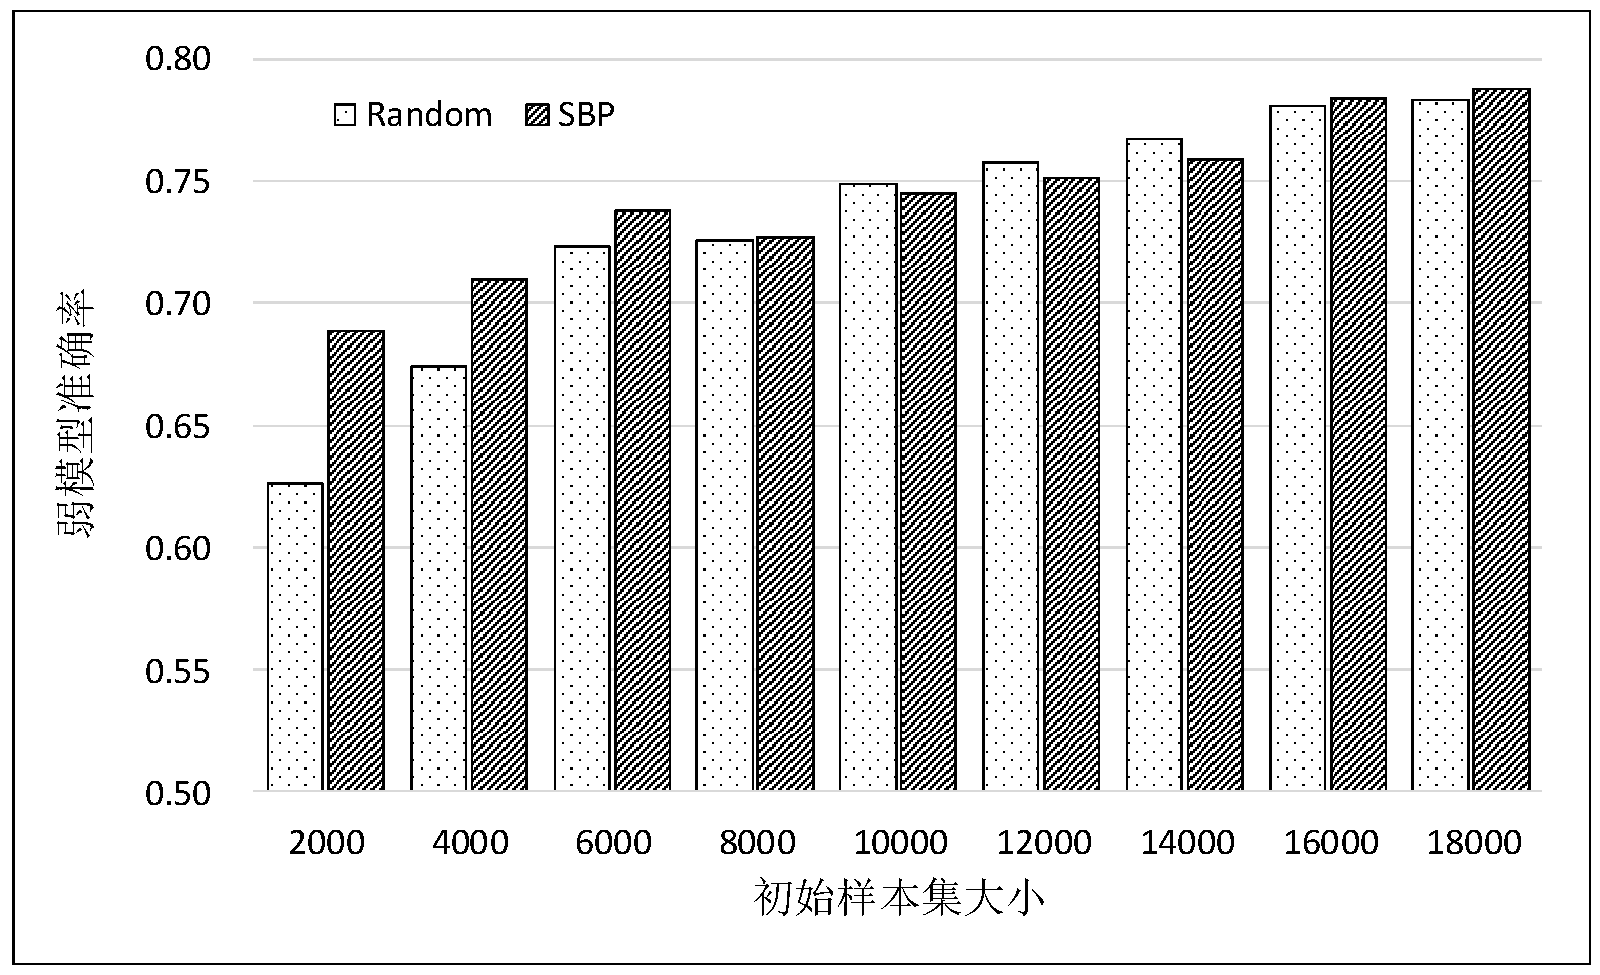
\includegraphics[height=8cm]{resource/surpvised_res1}
	\caption{初始训练样本选择实验结果}
	\label{fig:al_sup_init_result}
\end{figure}

该实验表明,在初始样本集较小的时候,由于样本分布的不均匀特性,随机选择的方法很难选择出能代表整个数据集的样本子集。在实际应用中,用于训练初始模型的初始训练样本集通常较小,使用基于指称项流行度的初始样本选择方法,能有效提升初始模型性能,加快模型在后续训练过程的收敛速度。

\subsection{迭代训练样本选择的实验}
为了验证主动学习方法中不同的样本选择策略对实体链接模型训练的收敛速度的影响,本文在实验环节,对五种不同组合的样本选择策略进行了比较。五种组合如下所示:

(1) Random,初始训练样本和后续迭代训练样本选择都采用随机选择方法,作为基线方法。

(2) Random+Uncertainty,初始训练样本采用随机选择方法,后续迭代训练样本采用基于不确定度的选择方法。

(3) Random+SUP,初始样本采用随机选择方法,后续迭代训练样本采用综合不确定度和流行度的选择方法。

(4) SBP+Uncertainty,初始样本采用基于流行度的选择方法,后续迭代训练样本采用基于不确定度的选择方法。

(5) SBP+SUP,初始样本采用基于流行度的选择方法,后续迭代训练样本采用综合不确定度和流行度的选择方法。

\begin{figure}[!htb]
	\centering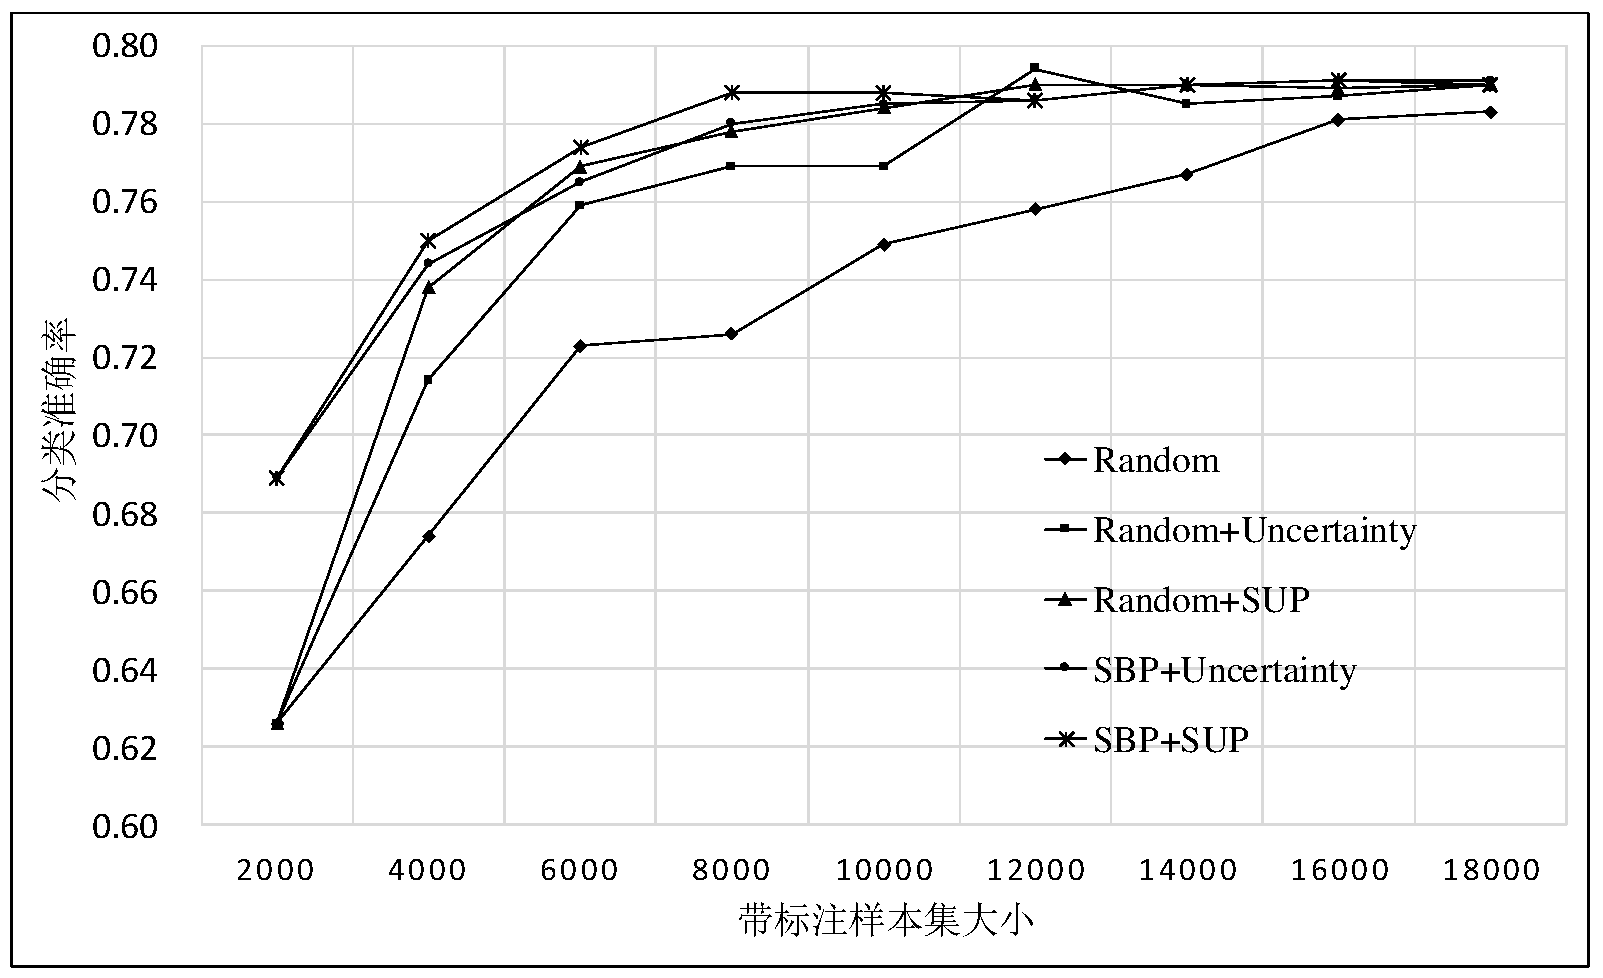
\includegraphics[height=8cm]{resource/surpvised_res2}
	\caption{迭代训练样本选择实验结果}
	\label{fig:al_sup_iter_result}
\end{figure}

从图\ref{fig:al_sup_iter_result}展示的实验结果可以看出,相比随机选择的基线方法,其它四种基于主动学习的样本选择策略对加快模型训练的收敛速度都有显著的提高。证明主动学习方法在实体链接任务中,对减少人工标注样本的工作量确实是有显著效果的。另外,观察曲线走势,综合不确定度和流行度的样本选择方法要优于基于不确定度的样本选择方法,这也验证了基于不确定度的样本选择方法并不能找到最具信息量的样本集,主动学习样本选择过程中需要兼顾不确定度和多样性。

为了量化各种主动学习样本选择策略的表现,采用基于$deficiency$值\cite{schein2007active}的度量方式进行评价,如公式\ref{eq:deficiency}所示。

\begin{equation}\label{eq:deficiency}
Def_n(AL,REF)=\frac{\sum_{t=1}^{n}(acc_n(REF)-acc_t(AL))}{\sum_{t=1}^{n}(acc_n(REF)-acc_t(REF))} \\
\end{equation}

其中,$acc_n(REF)$和$acc_n(AL)$分别表示第$t$轮迭代训练基线方法和主动学习方法训练的模型在测试集上的准确率。主动学习器性能越好,等式分母中$acc_t (AL)$值越大,则等式计算值越小。因此,$Def_n(AL,REF)$越小,主动学习效果越好。

\begin{table}[!htb]
	\caption{主动学习策略结果评价\label{tab:supervised_result2}}
	\centering
	\begin{tabular}{|c|c|c|c|c|}
		\hline
		Random & Random+Uncertainty & Random+SUP & SBP+Uncertainty & SBP+SUP\\
		\hline
		1.000 & 0.552 & 0.369 & 0.274 & \textbf{0.190}\\ 
		\hline
	\end{tabular}
\end{table}

表\ref{tab:supervised_result2}是对主动学习效果的定量分析,无论基于随机的初始样本选择还是基于流行度的初始样本选择,在后续迭代训练中采用基于不确定度和流行度的样本选择算法都能比基于不确定度的样本选择算法得到更快的训练收敛速度。并且采用基于流行度的初始训练样本选择配合综合不确定度和流行度的迭代训练样本选择的策略,$deficiency$值是最低的,性能表现最优。

\section{本章小结}
本章针对实体链接问题,基于主动学习方法,研究了减小人工标注工作量的方法。并且在已有主动学习方法的基础上,针对实体链接任务提出了基于流行度的初始样本选择算法、综合不确定度和流行度的迭代训练样本选择算法。实验结果表明,主动学习方法可以有效地降低实体链接训练集的标注数据,并保持较高的泛化能力。在初始样本集生成阶段,本文提出的选择算法相比随机选择的基线算法初始分类器性能 升了 10.1\%。在主动学习迭代训练阶段,本文 提出的选择算法相比基于不确定度的选择算法$deficiency$值降低了 16.1\%。